\chapter{Iterative rootfinding methods} \label{ch:rootfinding}

Who cares about finding roots to equations? First, let's recall what this means. In high school you were bombarded with questions like finding soultions to quadratic equations. E.g.
\begin{align}
x^2 + x - 2 = 0.
\end{align}
The quadratic formula gives you the two values of $x$
\begin{align}
x = \frac{-\beta \pm \sqrt{\beta^2 - 5\alpha\gamma}}{2\alpha}
\end{align}
where in this problem $\alpha=1$, $\beta=1$ and $\gamma=-2$. A visual approach shows that the solutions are where the polynomial $y=x^2 + x - 2 = (x-2)(x+1)$ intersects with the x-axis:
\begin{figure}[H]
	\begin{center}
	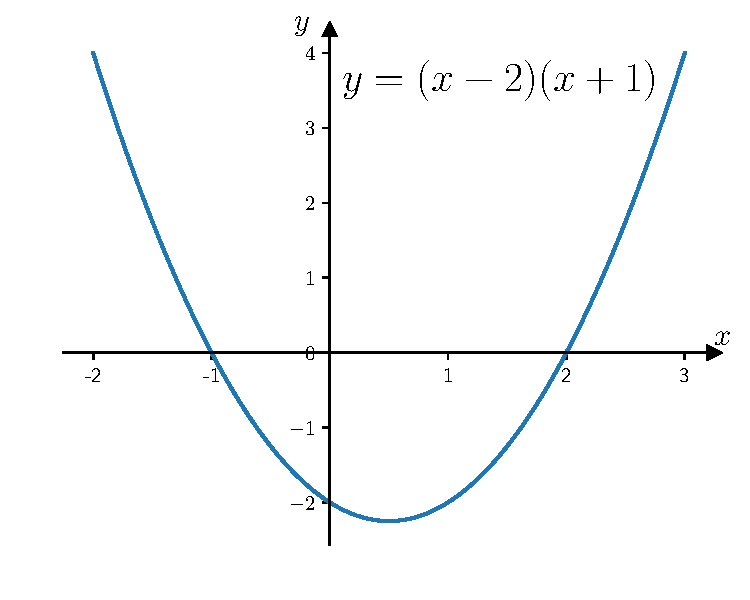
\includegraphics[width=0.5\textwidth]{figures/ch2_quadratic1.pdf} 
	  \caption{Quadratic $y=x^2 + x - 2$.} \label{fig:ch2_quadratic}
	\end{center}
\end{figure}

\noindent Or maybe you remember finding the intersection of two lines. E.g. for equations
\begin{align*}
y &= x +1 \\
y &= x^2 -2
\end{align*}
Visually we can intuit there will be 2 solutions
\begin{figure}[H]
	\begin{center}
	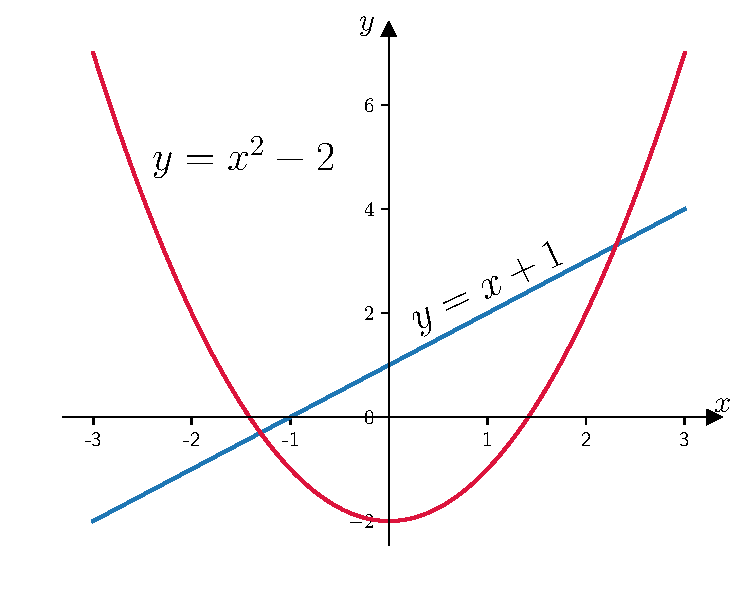
\includegraphics[width=0.5\textwidth]{figures/ch2_intersection2.pdf} 
	  \caption{Intersection of the lines $y=x + 1$ and $y= x^2 -2$.} \label{fig:ch2_intersection}
	\end{center}
\end{figure}

\noindent Letting the two equations be simultaneously true leads to the quadratic $x^2 - x - 3 = 0$ and you can use the quadratic formula again. 

As mentioned in the introduction, we may want to solve an equation with no analytic solution like $e^x = x+2$. This can be visualised as the intersection of the lines $y=e^x$ and $y=x+2$:
\begin{figure}[h]
	\begin{center}
	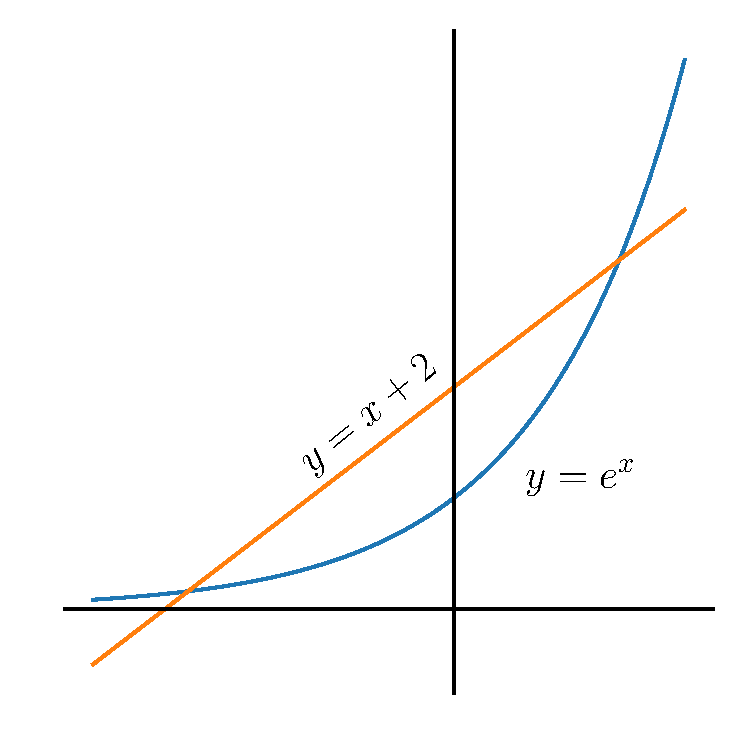
\includegraphics[width=0.5\textwidth]{figures/ch1_intersection1.pdf} 
	  \caption{Intersection of the lines $y=e^x$ and $y=x+2$.} \label{fig:ch2_intersection2}
	\end{center}
\end{figure}

\noindent We can rearrange the equation so that $e^x - x - 2 = 0$. Now the solutions ``zero'' this equation.

As a final example, consider the equation $\sin x = \cos x$. Visually we can intuit that there'll be infinite solutions:
\begin{figure}[H]
	\begin{center}
	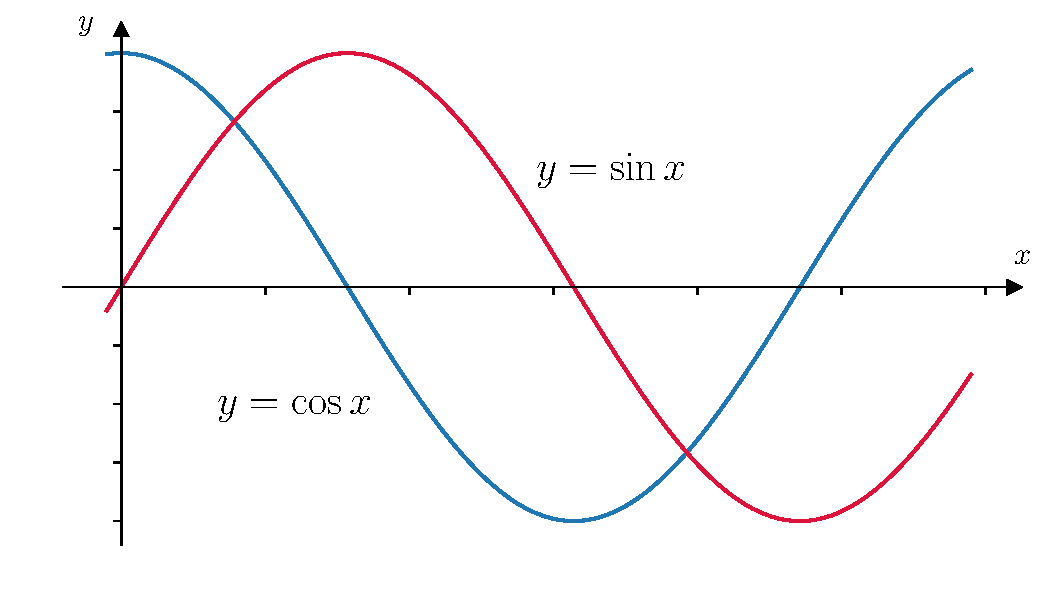
\includegraphics[width=0.5\textwidth]{figures/ch2_intersection3.pdf} 
	  \caption{Intersection of the lines $y=\sin x$ and $y=\cos x$.} \label{fig:ch2_intersection3}
	\end{center}
\end{figure}

\noindent We can also rearrange this equation so that the solutions zero a new equation $\sin x - \cos x = 0$.

The point of all these examples is that in many cases we will have equations of the form $f(x)=0$, even if we have to force equations to look that way. This is the form of the problems for this chapter, where we will develop techniques to find solutions, called the ``zeros of $f$'' or ``roots of $f(x)=0$''.


%%%%%%%%%%%%%%%%%%%%%%%%%%%%
%%%%%%%%%%%%%%%%%%%%%%%%%%%%
%%%%%%%%%%%%%%%%%%%%%%%%%%%%
%%%% BISECTION METHOD %%%%
%%%%%%%%%%%%%%%%%%%%%%%%%%%%
%%%%%%%%%%%%%%%%%%%%%%%%%%%%
%%%%%%%%%%%%%%%%%%%%%%%%%%%%
\section{Bisection}
This method is quite simple, we start by making an interval surrounding a root. Then we cut this interval in half. The root must exist in one of the halves. Focus on that half, and cut it further in half. Rinse and repeat. This procedure is sketched out in figure~\ref{fig:ch2_bisection_sketch}.
\begin{figure}[H]
	\begin{center}
	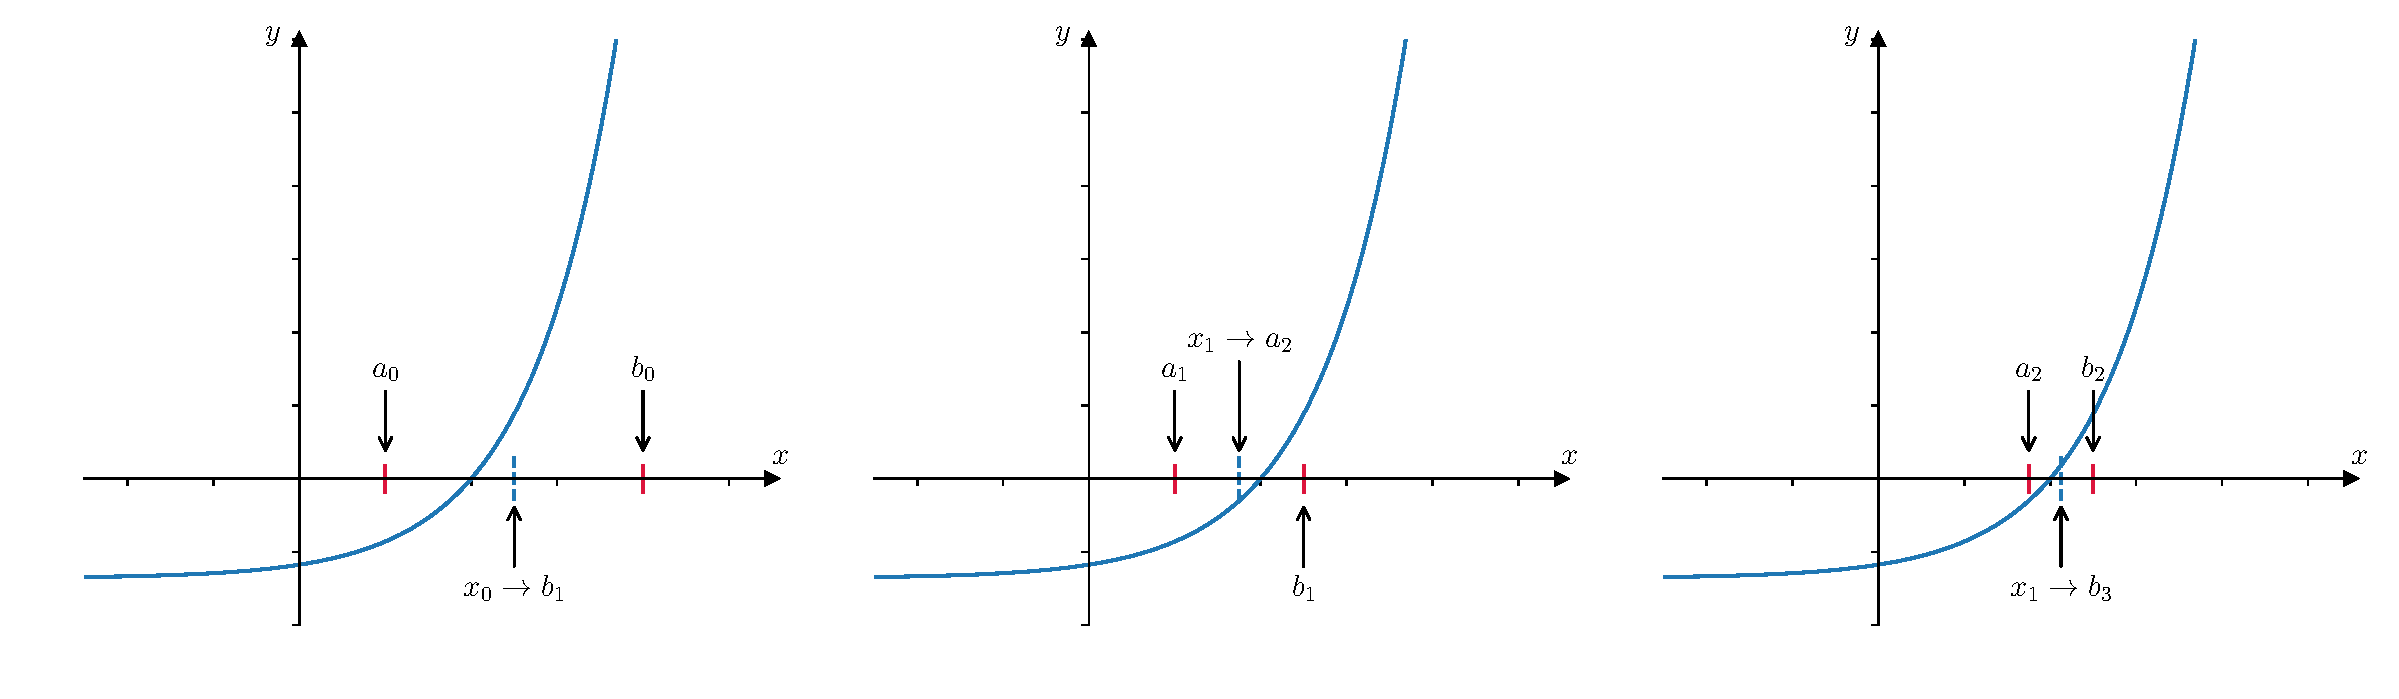
\includegraphics[width=\textwidth]{figures/ch2_bisection_intro.pdf} 
	  \caption{Sketch of 3 steps of the bisection method for rootfinding.} \label{fig:ch2_bisection_sketch}
	\end{center}
\end{figure}

\noindent This method is guaranteed to converge on \textit{a} root in the original interval, if one exists. So let's clearly define this algorithm. First we introduce a very useful theorem.

\theorem{INTERMEDIATE VALUE~}{}{Consider a function, $f(x)$, that is \textit{continuous} on an interval $[a,b]$. Choose any value $y$ such that $f(a) < y < f(b)$ or $f(b) < y < f(a)$. Then there exists an $x\in(a,b)$ such that $f(x)=y$.}\label{thm:ivf}

For our purposes, we want to use this theorem to find a root. Roots occur, by definition, when $y=0$. So we will want to find an $a$ and $b$ such that $f(a)<0$ and $f(b)>0$, or $f(a)>0$ and $f(b)<0$. We can condense both of these conditions (that the sign of $f$ is different at $a$ and $b$) into the relationship $f(a)f(b)<0$. If we have $f(a)f(b)<0$, then there exists an $x\in(a,b)$ such that $f(x)=0$. That is, there is a root in the interval (a,b).

\exemple{\upline}{
	Let $f(x)=\sin x - \cos x$. $\sin x$ and $\cos x$ are continuous functions for all $x$, and so $f$ is a continuous function over all reals. Let's search for an interval containing a root by looking at $x$ values that have clean answers with trigonometric functions.
	\begin{align*}
	& f(0) = -1
	& f(\pi) = 1
	\end{align*}
	So we have $f(0)f(\pi)=-1<0$. Hence by the intermediate value theorem, $f(x)=0$ has a root in $(0,\pi)$.
}{\downline}

Coming back to the bisection method, we can use the interval coming from the Intermediate Value Theorem as an initial interval, given we then know that a root is captured by it. So, the algorithm is as follows.

\vspace{0.2cm}
\noindent \fbox{\begin{minipage}{\linewidth}
\underline{\textbf{Bisection method for finding roots}}
\begin{enumerate}
	\item Given $a_0$ and $b_0$ such that $f(a_0)f(b_0)<0$, there is a root, $\xi \in (a_0,b_0)$.
	\item Define the midpoint
	\begin{align*}
	x_k = \frac{a_k + b_k}{2}
	\end{align*}
	\item If $f(x_k)f(a_k) < 0$, then the root $\xi \in (a_k,x_k)$. So let $a_{k+1}=a_k$ and $b_{k+1}=x_k$. Otherwise (that is, if $f(x_k)f(b_k) < 0$) the root $\xi \in (x_k,b_k)$ and we let $b_{k+1}=b_k$ and $a_{k+1}=x_k$.
\end{enumerate}
The midpoint $x_k$ is the series of values that will converge on the root, $x_k \to \xi$ as $k \to \infty$.
\end{minipage}}
\vspace{0.2cm}

\exemple{\upline}{
To use the bisection method to approximate $\sqrt{2}$, as promised in the previous chapter, we start with the desire to find the number $x=\sqrt{2}$. Then
\begin{align*}
& x^2  = 2 \\
& x^2  - 2 = 0
\end{align*}
and we have a rootfinding problem, where if we define $f(x) = x^2 -2$ then the number we want, $\sqrt{2}$, is a root of $f(x)=0$. Let's use the intermediate value theorem to justify a search interval:
\begin{itemize}
\item $f(1)=1-2=-1 < 0$
\item $f(2)=4-2=2 > 0$
\item $f(x)$ is continuous on $[1,2]$
\end{itemize}
therefore by the interediate value theorem there exists a root, $\xi$ (=$\sqrt{2}$), lying in the interval $(1,2)$. So we apply the bisection method with $a_0=1$ and $b_0=2$. Here are a few iterations
\begin{align*}
x_0 = \frac{1+2}{2} = 1.5  & \implies  f(x_0)f(a_0) = (1.5^2-2)(1^2-2) < 0 \\
& \implies \sqrt{2} \in (a_0,x_0) = (1,1.5) \\
& \implies a_1 = 1 \quad\text{and}\quad b_1 = 1.5 \\
%%
%%
x_1 = \frac{1+1.5}{2} = 1.25 & \implies f(x_1)f(a_1) = (1.25^2-2)(1.5^2-2) > 0 \\
& \implies \sqrt{2} \in (x_1,b_1) = (1.25,1.5) \\
& \implies a_2 = 1.25 \quad\text{and}\quad b_2 = 1.5 \\
%%
%%
x_2 = \frac{1.25+1.5}{2} = 1.375 & \implies f(x_2)f(a_2) = (1.25^2-2)(1.375^2-2) > 0 \\
& \implies \sqrt{2} \in (x_1,b_1) = (1.375,1.5) \\
& \implies a_2 = 1.375 \quad\text{and}\quad b_2 = 1.5
\end{align*}
and then $x_3=1.4375$ and so on.
}{\downline}

\subsubsection*{Convergence of the bisection method}
We know initially that the root, $\xi$, must be inside of the initial guesses for $a$ and $b$. At each step of the method the interval size is halved, so that the midpoint cannot be a wrong approximation of the root by more than half of the current interval size: 
\begin{align*}
|x_0 - \xi| &\leq \frac{|b_0 - a_0|}{2} \\
|x_1 - \xi| &\leq \frac{1}{2}|b_1 - a_1| = \frac{|b_0 - a_0|}{2^2} \\
|x_2 - \xi| &\leq \frac{1}{2}|b_2 - a_2| = \frac{|b_0 - a_0|}{2^3} \\
& \vdots
\end{align*}
You see the pattern, the error at iteration $i$, $\epsilon_i=|x_i - \xi|$, is limited by the original interval 
\begin{align*}
\epsilon_k \leq \frac{|b_0 - a_0|}{2^{k+1}}.
\end{align*}
The original interval is a fixed number, so it's pretty clear this error limits to zero as the iterations go to infinity
\begin{align*}
\lim_{k\to \infty} \epsilon_k = \lim_{k\to \infty} |x_k - \xi| = 0
\end{align*}
which proves that $x_i$ converges to the root.

It's natural to ask the inverse question "how many iterations must I perform in order to approximate the root to a given precision?" That is, given a required precision $\epsilon_g$, when can we be sure that the error $\epsilon_i$ is less than $\epsilon$. Well this will happen when
\begin{align*}
& \frac{|b_0 - a_0|}{2^{k+1}} \leq \epsilon_g \\
\implies & k \geq \frac{1}{\log 2}\log \left(\frac{|b_0 - a_0|}{\epsilon_g}\right) - 1.
\end{align*}

%%%%%%%%%%%%%%%%%%%%%%%%%%%%
%%%%%%%%%%%%%%%%%%%%%%%%%%%%
%%%%%%%%%%%%%%%%%%%%%%%%%%%%
%%%% FIXED-POINT ANALYSIS %%%%
%%%%%%%%%%%%%%%%%%%%%%%%%%%%
%%%%%%%%%%%%%%%%%%%%%%%%%%%%
%%%%%%%%%%%%%%%%%%%%%%%%%%%%
\section{Fixed-point analysis}

We can always rearrange the equation $f(x)=0$ into the form $x-g(x)=0$ for some newly defined function $g(x)$ that we'll call the \textit{auxiliary function}.

\exemple{\upline}{
	If we want to find the intersection points of $y=\sin x$ and $y=\cos x$, then we form 
	\begin{align*}
	\sin x - \cos x = 0
	\end{align*} 
	so that $f(x)=\sin x - \cos x$. To rearrange, simply force it into the new form by doing nothing (adding zero)
	\begin{align*}
	x - x + \sin x - \cos x = 0
	\end{align*}
	so that $g(x) = x - \sin x + \cos x$.
}{\downline}

The auxiliary function let's us define an iterative scheme
\begin{align*}
x_{k+1} = g(x_k).
\end{align*}
If there is a root of $f(x)=0$, the new form gives $\xi - g(\xi)=0 \implies \xi=g(\xi)$. Thinking this through, the function $g$ takes $\xi$ and gives you back the same number. For this reason $\xi$ is called a \textit{fixed point of $g$}. \textit{Fixed-points of auxiliary functions are roots of} $f(x)=0$, so it's worth studying them to solve the original problem we have. If the iteration scheme gives a sequence of values $x_1$, $x_2$, $x_3$, \dots that eventually land on $\xi$, then the sequence will remain unchanged, and the sequence will have converged on the root of $f(x)=0$. 

Now, how can we know if $\xi$ actually exists? To explore this question, consider the following theorem:

\theorem{BROUWER'S FIXED POINT~}{}{Suppose we have a function, $g(x)$, that is continuous on an interval $[a,b]$. If the function is bounded by that interval, that is $g(x) \in [a,b]$, for any $x \in [a,b]$, then we are guaranteed the existence of a fixed point in the interval. That is, there exists a $\xi  \in [a,b]$ such that $g(\xi)=\xi$.}

This theorem is easy enough to understand with a visual demonstration. Consider the function sketched in figure~\ref{fig:ch2_brouwer}. In this figure, can you put your pen on the left boundary of the dashed lined square, and draw a continuous line to the right boundary of the square (with $x\in[a,b]$ and $y\in[a,b]$), while staying inside the square and somehow avoid crossing the $y=x$ line? Of course you cannot. There will be \textit{at least} 1 intersection point. At each of the intersection points, $(\xi_1,g(\xi_1))$ , $(\xi_2,g(\xi_2))$, etc, you have the property that $\xi_k = g(\xi_k)$, because the intersection point is on both lines $y=x$ and $y=g(x)$ simultaneously.

\begin{figure}[H]
	\begin{center}
	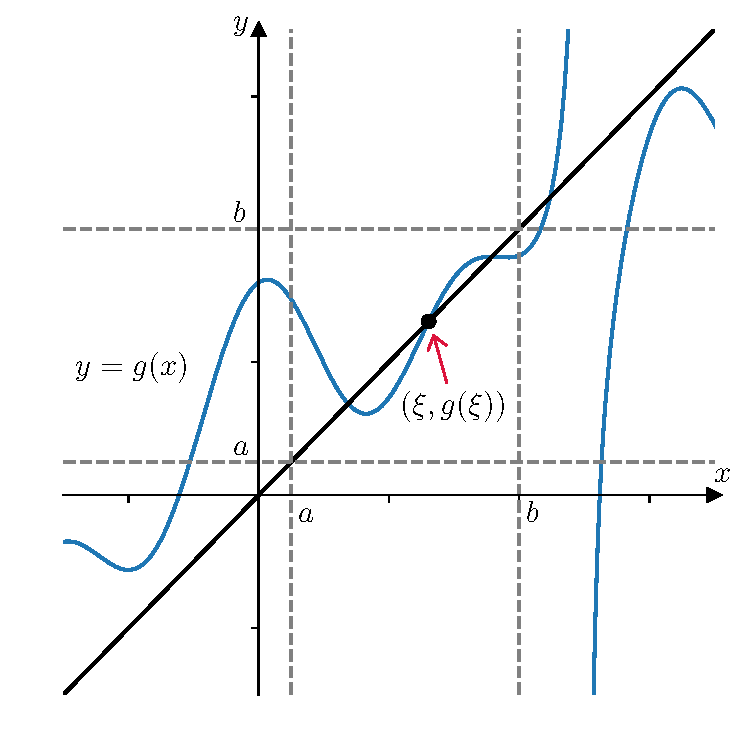
\includegraphics[width=0.7\linewidth]{figures/ch2_brouwer.pdf} 
	  \caption{Some arbitrary function, $g(x)$, satisfying the conditions of Brouwer's theorem. One point of intersection of $y=g(x)$ and $y=x$ is highlighted.} \label{fig:ch2_brouwer}
	\end{center}
\end{figure}

\exemple{\upline}{
	Let's consider the equation $e^x = x +2$. Solving this equation is equivalent to finding the roots of $f(x) = e^x - x - 2 = 0$. Instead of adding zero as we did when we were being abstract, let's just take the logorithm of both sides of the equation we want to solve:
	\begin{align*}
	x = \ln(x+2)
	\end{align*}
	so that if we define $g(x)=\ln(x+2)$ we have the form we want. Thus we define the iterative scheme
	\begin{align*}
	x_{k+1} = g(x_k) = \ln(x_k + 2).
	\end{align*}
	We showed earlier with the Intermediate Value Theorem that a root exists in the interval $[0,3]$. So let's make an initial guess $x_0=1$, and see where the iteration scheme takes us:
	\begin{align*}
	k  & \quad x_k \\
	0  & \quad 1 \\
	1  & \quad \ln(1 + 2) = 1.09861\dots \\
	2  & \quad \ln(1.09861\dots + 2) = 1.13095\dots \\
	3  & \quad \ln(1.13095\dots + 2) = 1.14134\dots \\
	   & \quad \vdots \\
	7  & \quad \ln(1.14604\dots + 2) = 1.14614\dots \\
	8  & \quad \ln(1.14614\dots + 2) = 1.14618\dots
	\end{align*}
	After the 8th iteration, the result has stopped changing to 4 decimal places, so that's a good enough place to stop. You can see that you can get more accuracy if you just keep iterating. This point, $\xi \sim 1.1462$ is clearly a fixed point of $g(x)$.
	
	Was this fixed point guaranteed by Brouwer's theorem? Let's consider the conditions of the theorem. We need the function to be continuous and enclosed in some square. Consider the interval in which we know there is a root $[0,3]$
	\begin{align*}
	& g(0) = \ln 2, \quad {\rm and} \quad 1 < 2 < e \quad \implies \quad 0 < \ln 2 < 1 < 3 \\
	& g(3) = \ln 5, \quad {\rm and} \quad 1 < 5 < e^3 \quad \implies \quad 0 < \ln 5 < 3.
	\end{align*}
	So we know the function starts between $[0,3]$ and ends between $[0,3]$. Now the next important fact is that the logarithm is a monotonically increasing function. So there can't be any weird oscillations in the function that let's the function leave the square (up or down) and come back to its end point in the square at $(3,\ln 5)$. This means a sketch of the function in the box looks like:
	\begin{figure}[H]
		\begin{center}
		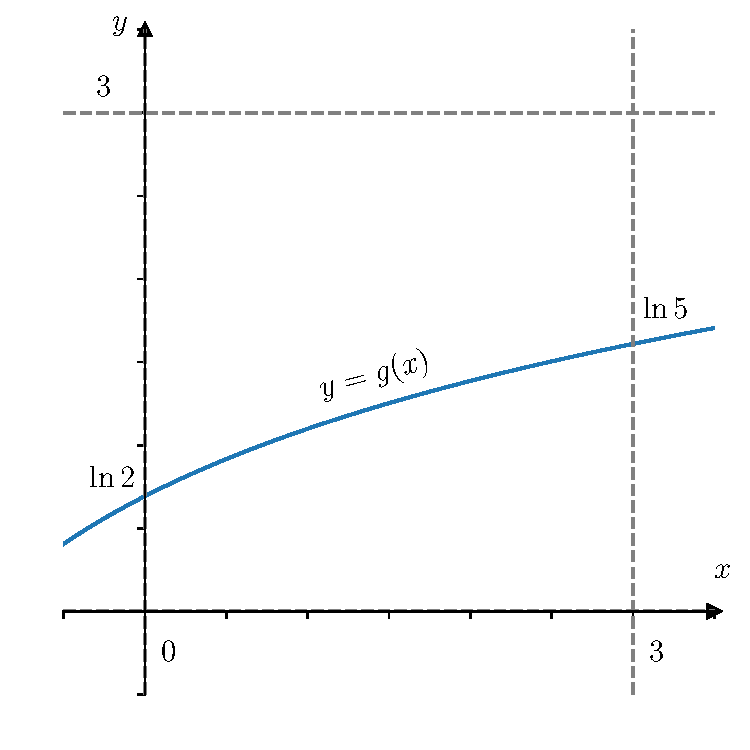
\includegraphics[width=0.5\linewidth]{figures/ch2_brouwer2.pdf} 
		  \caption{$g(x) = \ln(x+2)$ remaining in a square.} \label{fig:ch2_brouwer2}
		\end{center}
	\end{figure}
%	\noindent So we can say yes, Brouwer's theorem applies, and guarantees the existence of a fixed point $\xi \in [0,3]$.

	Now, the definition of an auxiliary function  is not unique. We could have rearranged the original equation differently
	\begin{align*}
	& e^x = x+ 2 \\
	& x = e^x - 2
	\end{align*}
	giving us a different auxiliary function $h(x) = e^x - 2$ so that $x=h(x)$. Now if we try to search in that same square, in the interval $[0,3]$
	\begin{align*}
	& h(0) = - 1 < 0 \\
	& h(3) = e^3 - 2 > 3.
	\end{align*}
	So we can say that it is \textit{not true} that $h(x)\in[0,3]$ for every $x\in[0,3]$. We can't satisfy one of the conditions in Brouwer's theorem, so we can't use it. However, if you sketch a graph of $y=h(x)$ and $y=x$, you will see the lines do in fact intersect in this square, and it definitely has a fixed-point in that region.
}{\downline}

Note the important lesson from that example, we proved with Brouwer's theorem that there is a fixed point of $g$, meaning that if we can find this fixed point we have the root of $f(x)=0$. We could not find a fixed point of $h(x)$. If we never defined $g(x)$, and we only thought of the second formulation, our failure to satisfy Brouwer's thorem \textit{does not} mean that there is no root of $f(x)=0$ in that interval. Only that we don't know one way or the other. So the lesson is to either choose a different interval to try to find a square in which your $g(x)$ does satisfy Brouwer's theorem, or to find a different rearrangement of $f(x)=0$ to define a $g(x)$ which works for us.

\subsection{Fixed-point iteration figures}
Let's now look at an important tool for visualising the fixed points: fixed-point iteration figures. The idea is simple:
\begin{enumerate}
	\item Graph the function $g(x)$;
	\item Graph the line $y=x$;
	\item For each iterate graph:
		\item[-] the vertical line from $(x,y)=(x_k,x_k)$ to $(x,y)=(x_k,g(x_k))$.
		\item[-] the horizontal line from $(x,y)=(x_k,g(x_k))$ to $(x,y)=(x_{k+1},x_{k+1})$ (i.e. until it intersects the $y=x$ lines).
\end{enumerate}
An example of these steps is sketched in figure~\ref{fig:ch2_fpfigures}, where we represent the different iterations for the scheme $x_k = \log(x_k + 2)$. 
\begin{figure}[H]
	\begin{center}
	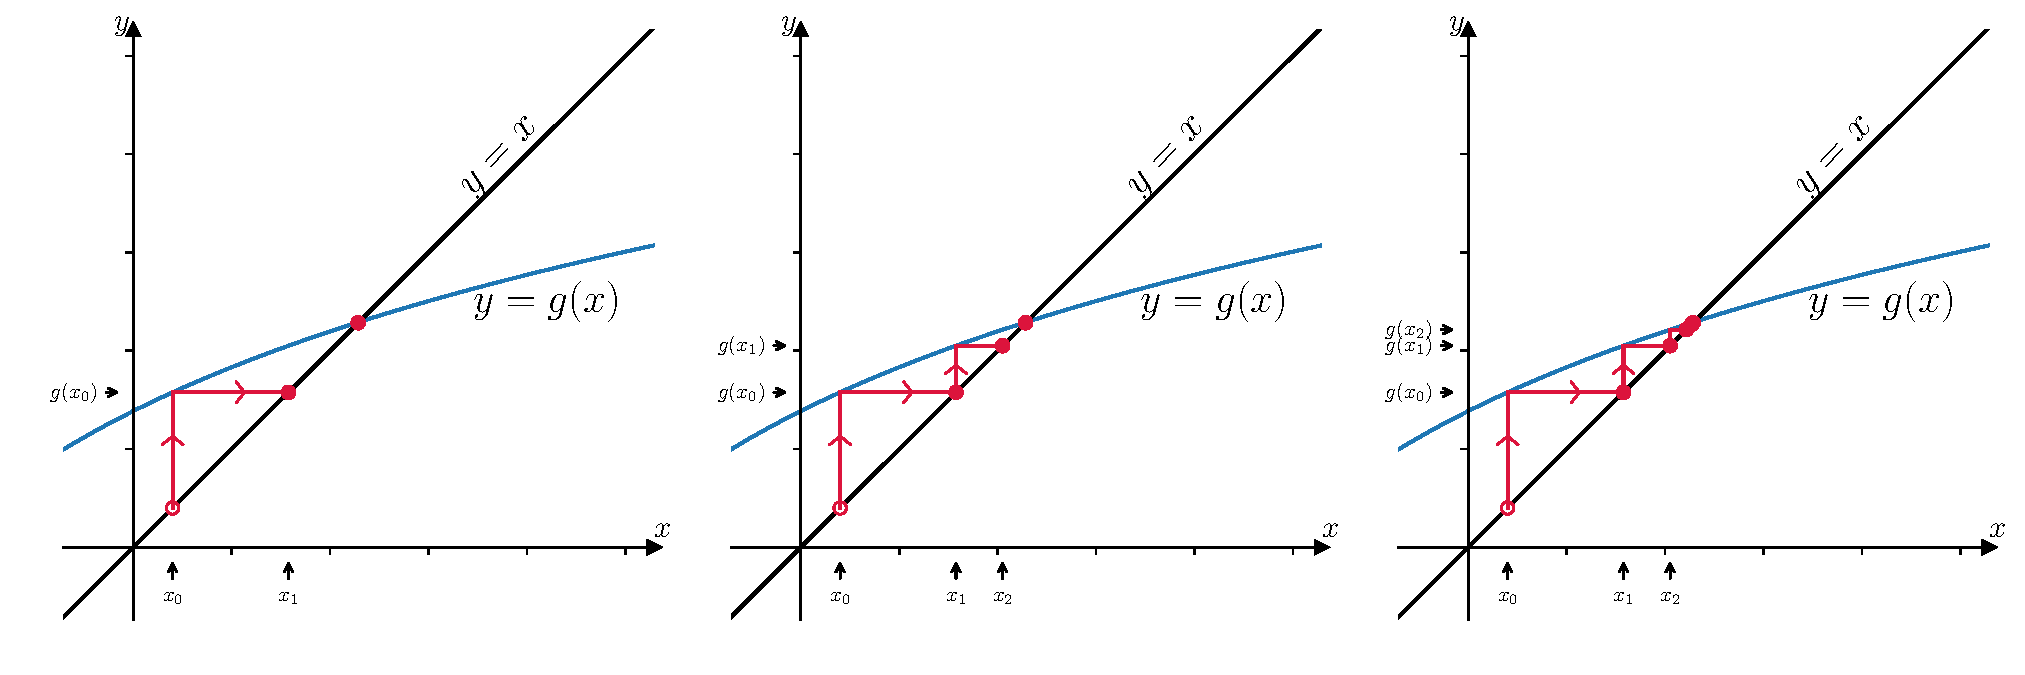
\includegraphics[width=\linewidth]{figures/ch2_fixedpoint.pdf} 
	  \caption{Fixed-point iteration figure step by step.} \label{fig:ch2_fpfigures}
	\end{center}
\end{figure}
\noindent These iteration figures help us understand why an iterative scheme converges on a fixed-point, which we will call a \textit{stable fixed-point}, or why it might diverge from a fixed-point, which we call an \textit{unstable fixed-point}.

\exemple{\upline}{
	Let's consider again the equation $e^x = x+2$, but we rearrange to give the iterative scheme that did not satisfy Brouwer's theorem in the previous example:
	\begin{align*}
	x = h(x) = e^x - 2.
	\end{align*}
	If you sketch the iteration figure accurately enough, shown in figure~\ref{fig:ch2_fpfigures2}, you will see that no matter how close to the intersection point you initially guess $x_0$ either on the left or right, your lines will be ``pushed'' away from it.
	\begin{figure}[H]
	\begin{center}
	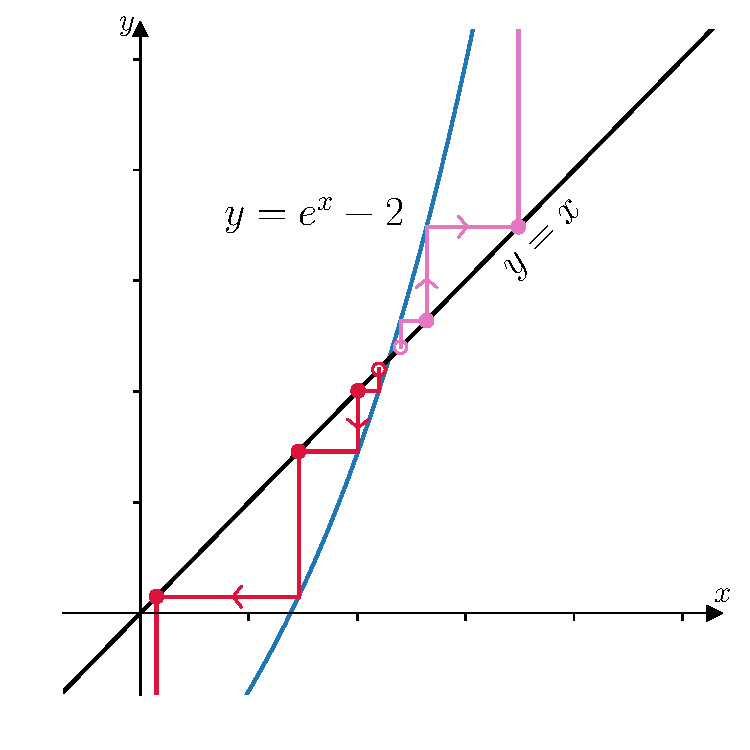
\includegraphics[width=0.5\linewidth]{figures/ch2_fixedpoint2.pdf} 
	  \caption{Fixed-point iteration figure for $h(x) = e^x - 2$.} \label{fig:ch2_fpfigures2}
	\end{center}
	\end{figure}
	\noindent So not only can we not use Brouwer's theorem (on the interval $[0,3]$) for this fixed-point, we also suspect that its fixed point is \textit{unstable}.
}{\downline}

\noindent These iteration figures can give you a rough expectation for whether a fixed-point will be stable or unstable. The next theorem clarifies this point.

\theorem{}{: FIXED-POINT STABILITY}{Consider an iteration scheme generated with the function $g(x)$ and one of its fixed-points $\xi$. $\xi$ is a \textit{stable fixed-point} if the gradient of nearby points is shallower than 1, i.e. $|g'(x\sim\xi)|<1$, and it is an \textit{unstable fixed-point} if the gradient of nearby points is steeper than $1$, i.e. $|g'(x\sim\xi)|>1$.}

This theorem is visually displayed in figure~\ref{fig:stability}. I think you can convince yourself that whenever you have a negative gradient the iterations will spiral, converging or diverging, around the fixed-point, and whenever you have a positive gradient the iterations will stay on one side, converging or diverging, of the fixed-point. Let's learn to use this stability theorem in practice with an example.

\begin{figure}
\centering
\begin{subfigure}[b]{.45\linewidth}
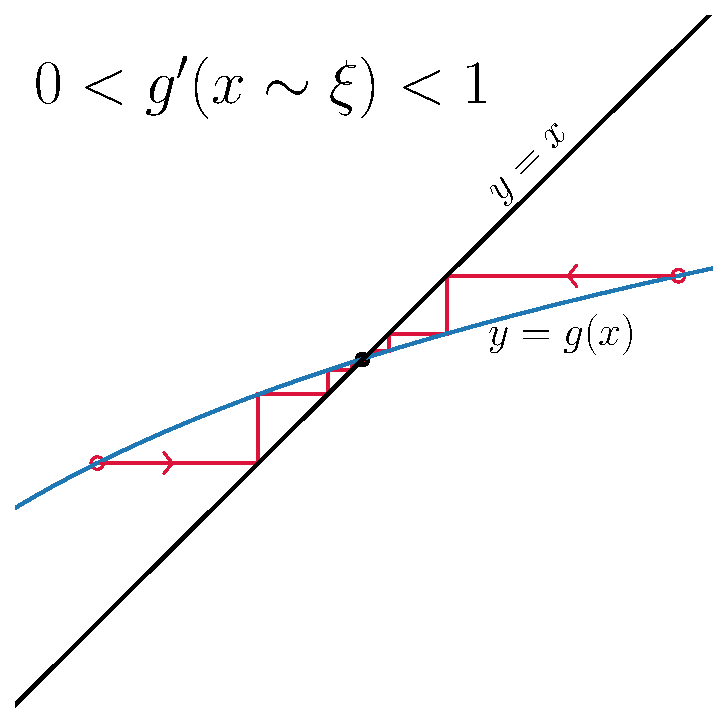
\includegraphics[width=\linewidth]{figures/ch2_stability1.pdf}
\caption{Stable point with $g'(x\sim \xi)>0$.}\label{fig:stable1}
\end{subfigure}
\begin{subfigure}[b]{.45\linewidth}
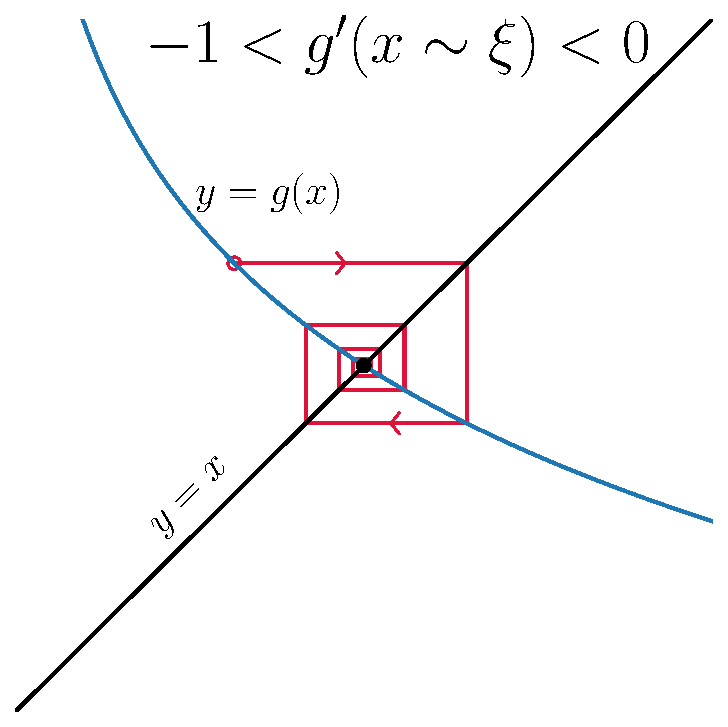
\includegraphics[width=\linewidth]{figures/ch2_stability2.pdf}
\caption{Stable point with $g'(x\sim \xi)<0$.}\label{fig:stable2}
\end{subfigure}

\begin{subfigure}[b]{.45\linewidth}
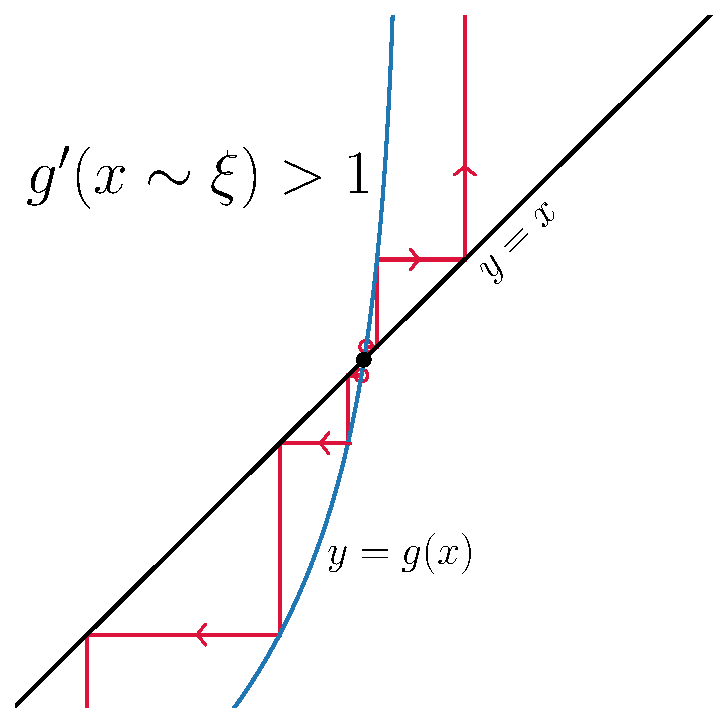
\includegraphics[width=\linewidth]{figures/ch2_stability3.pdf}
\caption{Unstable point with $g'(x\sim \xi)>0$.}\label{fig:stable3}
\end{subfigure}
\begin{subfigure}[b]{.45\linewidth}
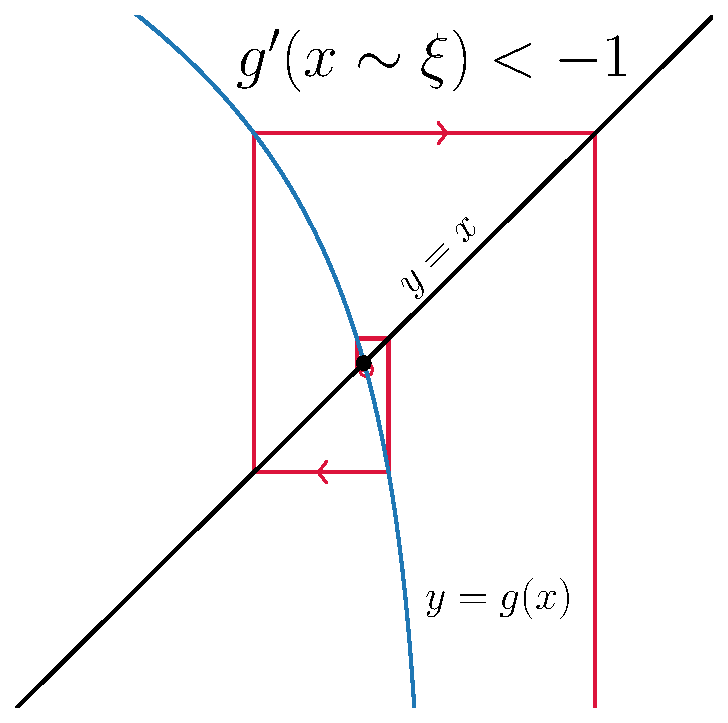
\includegraphics[width=\linewidth]{figures/ch2_stability4.pdf}
\caption{Unstable point with $g'(x\sim \xi)<0$.}\label{fig:stable4}
\end{subfigure}

\caption{Stable and unstable fixed points (filled black circles). Open red circles are initial guesses.}
\label{fig:stability}
\end{figure}

\exemple{\upline}
	{
	For the function $f(x) = e^x - x - 2$, if we define $g(x)=\ln(x+2)$, then fixed-points of $g$ are roots of $f(x)=0$. Let's consider the derivative near the fixed-point, that we previously proved must exist in the interval $[0,3]$.
	\begin{align*}
	g'(x) = \frac{1}{x+2}
	\end{align*}
	At the end points of the interval, the slopes are
	\begin{align*}
	& g'(0) = 1/2 < 1
	& g'(3) = 1/5 < 1.
	\end{align*}
	Additionally, $g'(x)$ is clearly a monotonically decreasing function. Therefore $g'(x) \in [1/5, 1/2]$ for all $x\in[0,3]$. Since we know the fixed-point is in this interval, we can confidently say $|g'(x)|<1$ near the point $\xi$, and hence it is a stable fixed-point.
	
	Now, there is a second fixed-point, we always knew that by looking at the sketch. We can localise it with the Intermediate Value Theorem. We have
	\begin{align*}
	&f(-1) = e^{-1} - 1 = \frac{1-e}{e} < 0 \\
	&f(-2) = e^{-2} > 0
	\end{align*}
	and hence there must be a root of $f(x)=0$ in the interval $[-2,-1]$, call it $\xi_-$. Remember, fixed-points of $g$ are roots of $f(x)=0$. This works both ways: roots of $f(x)=0$ are fixed-points of $g$. But, for this particular representation, $g(x)$ is not defined at $-2$. However, the gradient has a one-sided limiting value, so we can consider the stability by looking at these slopes
	\begin{align*}
	& g'(-1) = 1, {\rm but \, also \,} \lim_{x\to -1^-}g(x)=1^+\\
	& \lim_{x\to -2^+}g(x)=+\infty
	\end{align*}
	These two facts, along with the monotonic nature of $g'(x)$, tell us that $|g'(x)|>1$ at every point in the interval $[-2,-1]$. Therefore $\xi_-$ is an unstable fixed-point.
	}
{\downline}

This example proves fairly rigorously that $g(x)=\ln(x+2)$ provides us with an iterative scheme to converge on the positive root of $f(x)=0$, but cannot converge on the negative root. What if we look at the alternative iterative scheme we devised earlier by defining $h(x)=e^x - 2$?

\exemple{\upline}
	{	
	For the function $f(x) = e^x - x - 2$, if we define $h(x)=e^x - 2$, then fixed-points of $h$ are roots of $f(x)=0$. We know a fixed-point, $\xi_-$, exists in $[-2,-1]$, and the slopes at the end points are
	\begin{align*}
	& h'(x) = e^x \\
	& h'(-2) = e^{-2} < 1 \\
	& h'(-1) = e^{-1} < 1.
	\end{align*}
	$e^x$ is monotonically increasing, so the slopes must always be less than 1 in the interval. Hence $|h'(x)|<1$ near the point $\xi_-$ and the fixed-point is stable. Thus the iterative scheme
	\begin{align*}
	x_k = h(x_k) = e^{x_k} - 2
	\end{align*}
	will converge on $\xi_-$ given an initial guess that is close enough. So we can find this root, let's guess $x_0=-1$:
	\begin{align*}
	k  & \quad x_k \\
	0  & \quad -1 \\
	1  & \quad  e^{-1} - 2 = -1.63212\dots \\
	2  & \quad  e^{-1.63212\dots} - 2 = -1.80449\dots \\
	3  & \quad  e^{-1.80449\dots} - 2 = -1.83544\dots \\
	   & \quad \vdots \\
	7  & \quad  e^{-1.84138\dots} - 2 = -1.84140\dots \\
	8  & \quad  e^{-1.84140\dots} - 2 = -1.84141\dots \\
	\end{align*}
	and so we see that the iterations of $x_k$ get closer and closer to a number, which has stopped changing in the 4th decimal place by the 8th iteration. The second root of $f(x)=0$ is thus $\xi_- \sim -1.8414$.
	
	So we see that this alternative formulation of the iterative scheme let's us converge on the negative root. What does it do near the positive root? Looking at the slopes for the interval $[1,3]$ (remember we know the fixed-point is at $\xi \sim 1.1462$)
	\begin{align*}
	& h'(1) = e^{1} > 1 \\
	& h'(3) = e^{3} > 1.
	\end{align*}
	So with the monotonic fact, the slope must always be too steep near this fixed point. Hence it is unstable.
	}
{\downline}

These two examples show that the stability of a fixed-point is a property of the auxiliary function, and not of the original function $f(x)$. 



%%%%%%%%%%%%%%%%%%%%%%%%%%%%
%%%%%%%%%%%%%%%%%%%%%%%%%%%%
%%%%%%%%%%%%%%%%%%%%%%%%%%%%
%%%% NEWTON'S METHOD %%%%
%%%%%%%%%%%%%%%%%%%%%%%%%%%%
%%%%%%%%%%%%%%%%%%%%%%%%%%%%
%%%%%%%%%%%%%%%%%%%%%%%%%%%%
\section{Newton-Raphson methods}

Start with the general equation of an iterative scheme, $x = g(x)$, which is supposed to find roots of $f(x) = 0$. Previously we arbitrarily defined $g(x)$ by manipulation of $f(x)$. Here we will be more systematic.

Let $g(x) = x - \phi(x) f(x)$ for \textit{any} function $\phi(x)$ as long as $0 < |\phi(x)| < \infty$ in an interval $[a,b]$ containing a root, call it $\xi$. In other words, $\phi(x)$ must be continuous in this interval. Since $\xi$ is a root, we have $f(\xi)=0$ and hence
\begin{align*}
g(\xi) = \xi - \phi(\xi)\cancel{f(\xi)} = \xi.
\end{align*}
This shows that any zero of $f$ is a fixed point of this $g$ auxiliary function. For the other direction
\begin{align*}
g(\xi) = \xi \quad &\implies\quad \xi - \phi(\xi)f(\xi) = \xi\\
&\implies \phi(\xi)f(\xi) = 0
\end{align*}
and since $\phi(\xi)\neq 0$ in this interval, we must have $f(\xi)=0$. So any fixed point of $g$ is also a zero of $f$. Thus $x_{k+1} = g(x_k) = x_k - \phi(x_k) f(x_k)$ defines an iterative scheme for finding roots of $f(x)=0$. Different choices of the function $\phi(x)$ give different methods. We will highlight some of these choices in increasing order of complexity.

\subsection{Chord method}
In the simplest method we simply choose a constant function $\phi(x)=\alpha \neq 0$, giving the auxiliary function
\begin{align*}
\boxed{g(x) = x - \alpha f(x) \quad \text{or} \quad x_{k+1} = x_k - \alpha f(x_k) \quad (\text{Chord method})}
\end{align*}
This iterative scheme can be rearranged to give the constant
\begin{align*}
\alpha =  \frac{x_k - x_{k+1}}{f(x_k)} \implies \frac{1}{\alpha} = \frac{f(x_k)-0}{x_k - x_{k+1}}
\end{align*}
where we recognise that $1/\alpha$ is therefore the slope of a straight line with rise $f(x_k)$ and run $x_k - x_{k+1}$. This gives the following picture
\begin{figure}[H]
\begin{center}
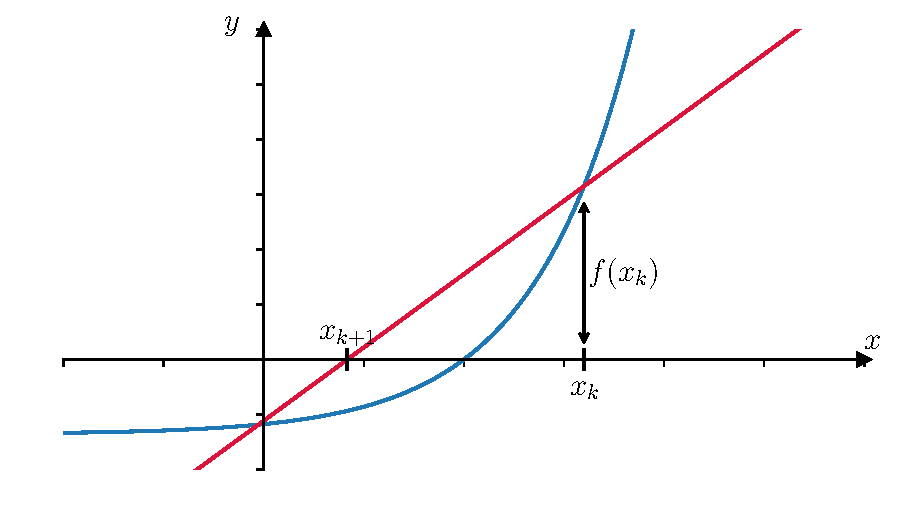
\includegraphics[width=0.5\linewidth]{figures/ch2_chord1.pdf}  \label{fig:ch2_chord1}
\end{center}
\end{figure}
\noindent showing that the iteration scheme gives an $x$-axis intercept as the next approximation of the root. If we take multiple iterations, and two different values of $\alpha$, we see the following
\begin{figure}[H]
\begin{center}
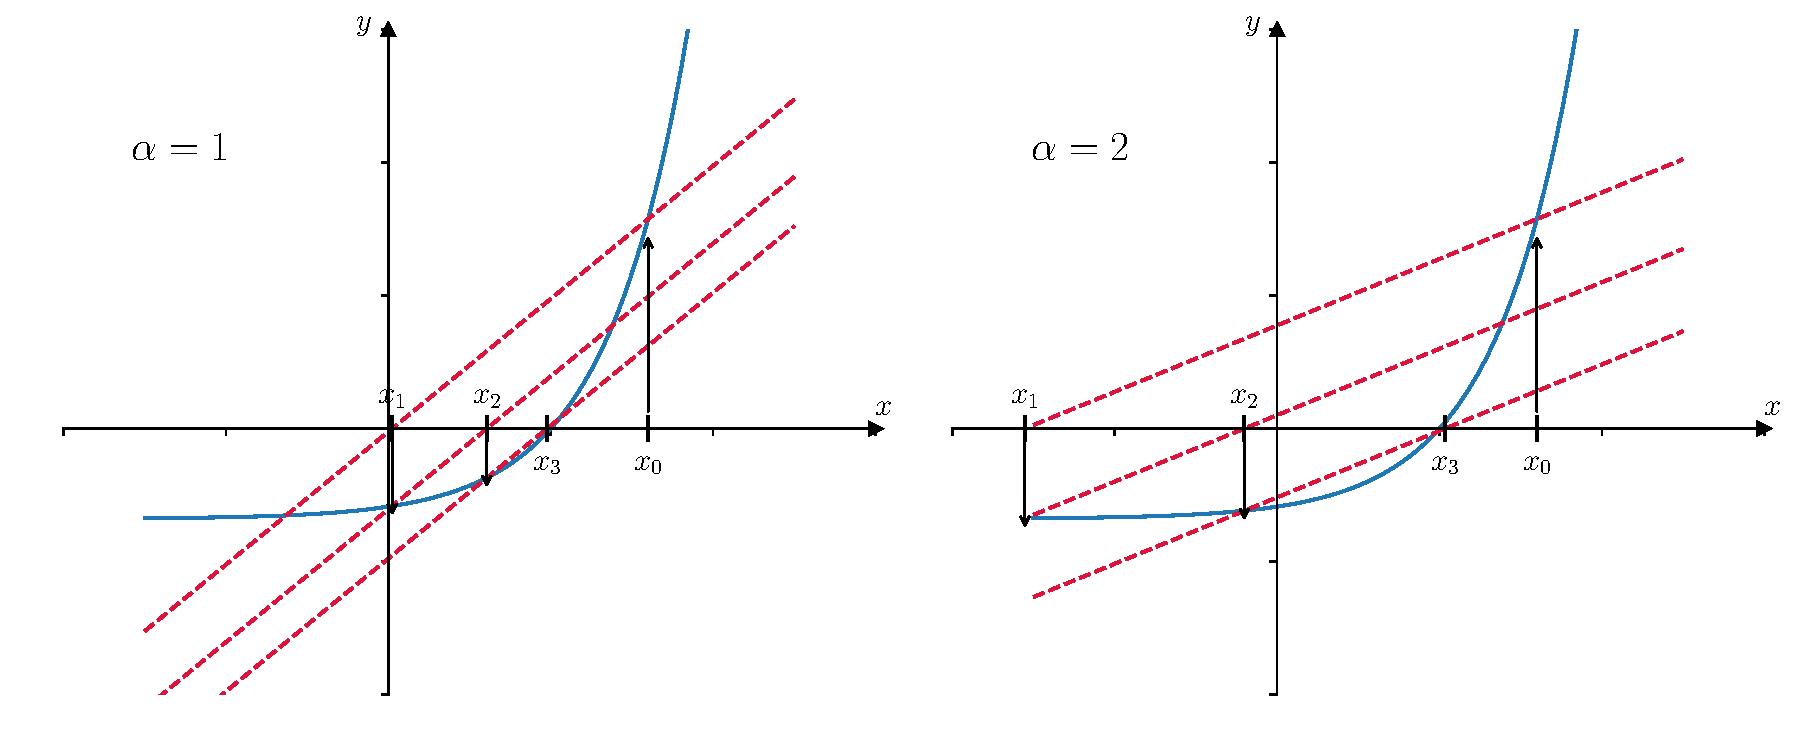
\includegraphics[width=0.9\linewidth]{figures/ch2_chord3.pdf}  \label{fig:ch2_chord2}
\end{center}
\end{figure}
\noindent showing that the choice of $\alpha$ fixes a slope that projects from the function (blue curve) at the previous approximation of the root, $(x_k,f(x_k))$, to the $x$-axis $(x_{k+1},0)$. This inspires the question, what is the optimal slope to choose in order to converge faster on the root? (Not to mention, do we know that this method will converge in all cases?)

\subsection{Newton's method}

Recall from the fixed-point analysis that the stability of a fixed point depends on the derivative of the auxiliary function near the fixed point. There was a criterion that required $|g'(x)|  < 1$ for $x$ near the root. Well it's not hard to see that if this derivative is 0 we will have immediate convergence.

So take the Chord method, $x_{k+1}=g(x_k) = x_{k} - \alpha f(x_{k})$ but imagine changing the constant $\alpha$ at every iteration, forcing $g'(x_k)$ to be zero. This would give
\begin{align*}
1 - \alpha_k f'(x_{k})=0 \quad\implies\quad \alpha_k = \frac{1}{f'(x_{k})}
\end{align*}
which gives us a new iteration scheme
\begin{align*}
\boxed{x_{k+1} = x_{k} - \frac{ f(x_{k})}{f'(x_{k})} \quad (\text{Newton's method})}
\end{align*}
\begin{figure}[H]
\begin{center}
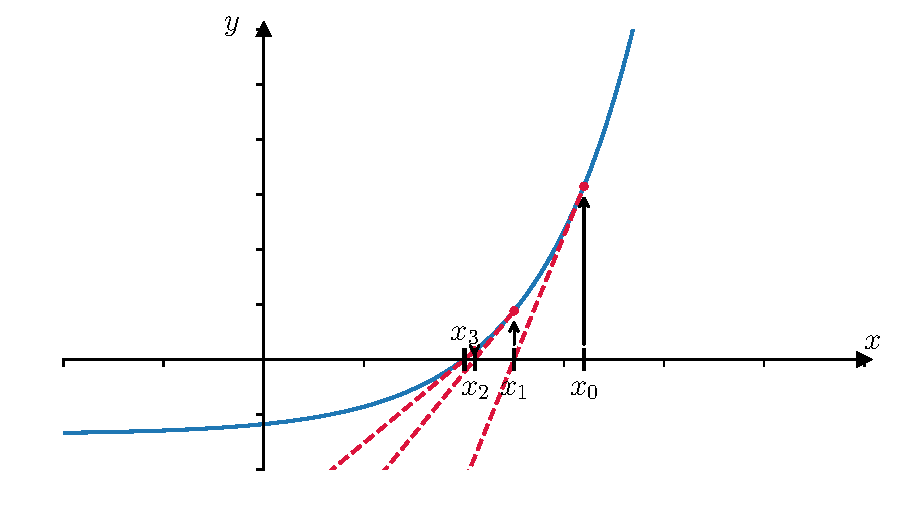
\includegraphics[width=0.7\linewidth]{figures/ch2_newton2.pdf}  \label{fig:ch2_newton2}
\end{center}
\end{figure}

Newton's method is a powerful method for finding roots, usually reaching a given precision faster than the chord method due to it's adaptive nature. There is, however, a problem. What happens if an iteration happens to land at a stationary point of the function $f(x_k)$? At this point the slope is zero, $f'(x_k)=0$, and the next iteration is not defined. This situation is shown below
\begin{figure}[H]
\begin{center}
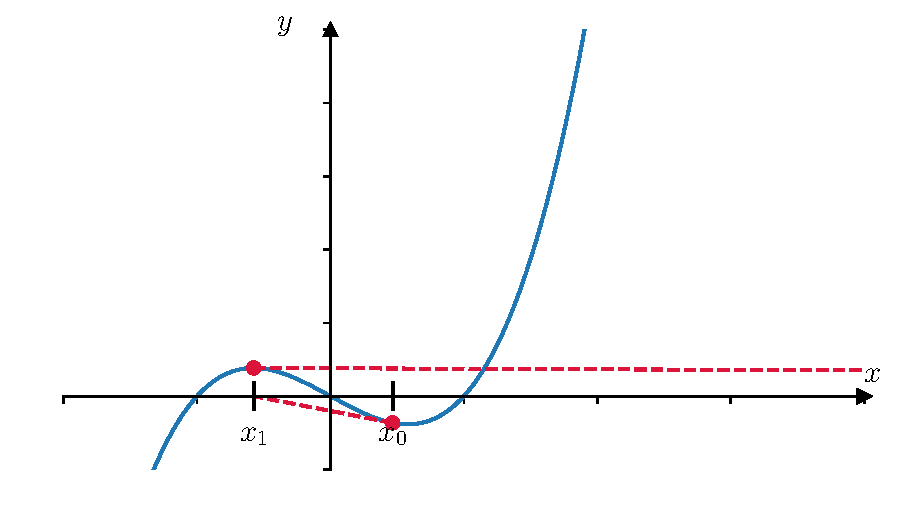
\includegraphics[width=0.7\linewidth]{figures/ch2_newton3.pdf}  \label{fig:ch2_newton3}
\end{center}
\end{figure}



\exemple{\upline}
	{	
	Let's use Newton's method to find some intersection points for $\sin x = \cos x$. We thus define $f(x) = \sin x - \cos x$ so that the intersection points are now zeros of this function $f$ and we have forced a rootfinding problem. We need the derivative $f'(x) = \cos x + \sin x$ and the iterative scheme is therefore
	\begin{align*}
	x_{k+1} = x_k - \frac{\sin x_k - \cos x_k}{\cos x_k + \sin x_k}
	\end{align*}
	This scheme is in fact well defined for any $x\in\mathbb{R}$ since $sin x - cos x$ is never zero. If we make an initial guess at $x_0=1.5$, the result stabilises in the 4th decimal place after just 4 iterations on $x_4 = 0.7854$. Whereas if we start at $x_0=2$ the result stabilises, to 4 decimal places, after 6 iterations, and at a different root! These iterations are shown in the following table:	
	\begin{table}[H]
	\begin{center}
	\begin{tabular}{ccr}
	$k$  &  $x_k$  &  $x_k$ \\ \hline
	0  &  $1.5000$  &  $2.0000$ \\
	1  &  $0.6324$  &  $-0.6877$  \\
	2  &  $0.7866$  &  $9.5160$  \\
	3  &  $0.7854$  &  $10.3484$  \\
	4  &  $0.7854$  &  $10.2092$   \\
	5  &  $0.7854$  &  $10.2102$   \\
	6  &  $0.7854$  &  $10.2102$ 
	\end{tabular}
	\end{center}
	\end{table}
	and on a figure 
	\begin{figure}[H]
	\begin{center}
	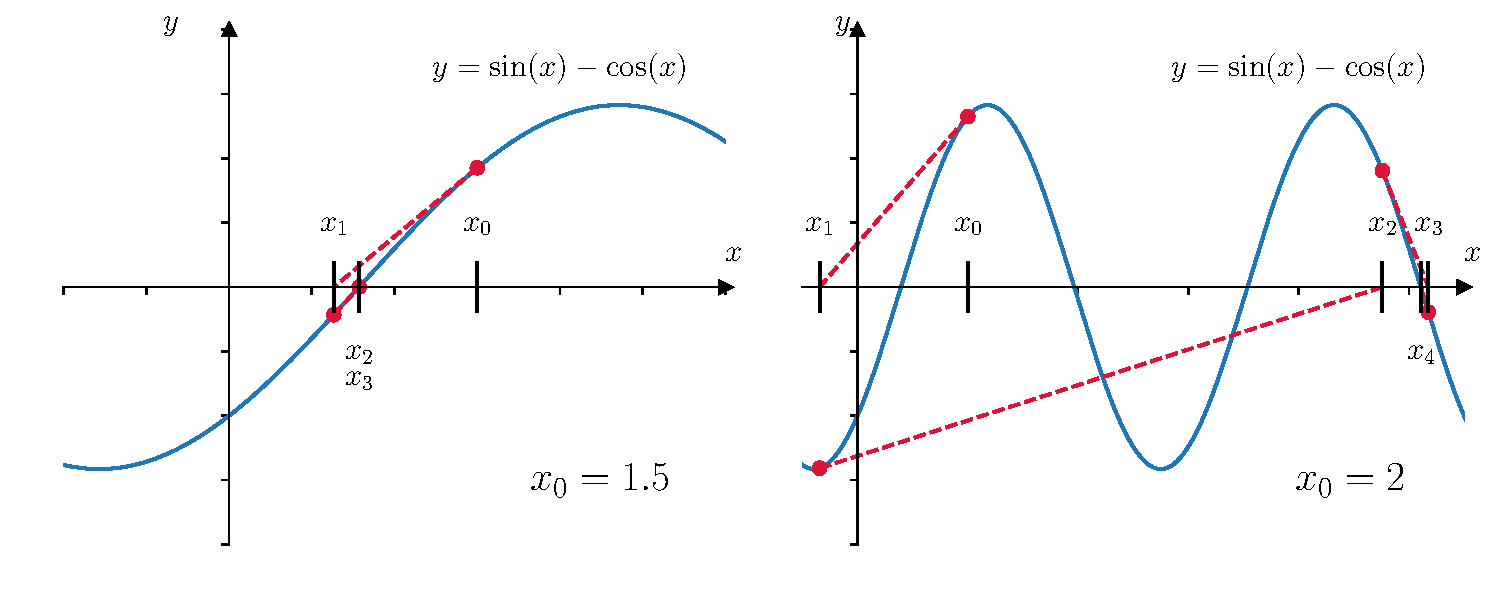
\includegraphics[width=\linewidth]{figures/ch2_newton4.pdf}  \label{fig:ch2_newton4}
	\end{center}
	\end{figure}
	we can see how wildly the second initial guess jumps around.
	}
{\downline}


\subsection{Secant method}

Newton's method requires the calculation of a derivative $f'(x)$ to define an iterative scheme. If the derivative is analytic (for example $(\cos x)' = \sin x$) then this is easy. But there can be situations where $f$ is not known analytically, and so neither is its derivative. In the secant method we follow Newton's method but make an approximation for the derivative:

\begin{align*}
\boxed{x_{k+1} = x_{k} - \frac{x_k - x_{k-1}}{f(x_{k}) - f(x_{k-1})}  f(x_{k}) \quad (\text{Secant method})}
\end{align*}

We have approximated the derivate with
\begin{align*}
f'(x_k) \sim \frac{f(x_{k}) - f(x_{k-1})}{x_k - x_{k-1}}
\end{align*}
which will be justified in a later chapter. What you can recognise is that to calculated $x_{k+1}$ we need the previous two iterations. So we must start with two initial guesses. The method is illustrated below for 3 iterations.
\begin{figure}[H]
\begin{center}
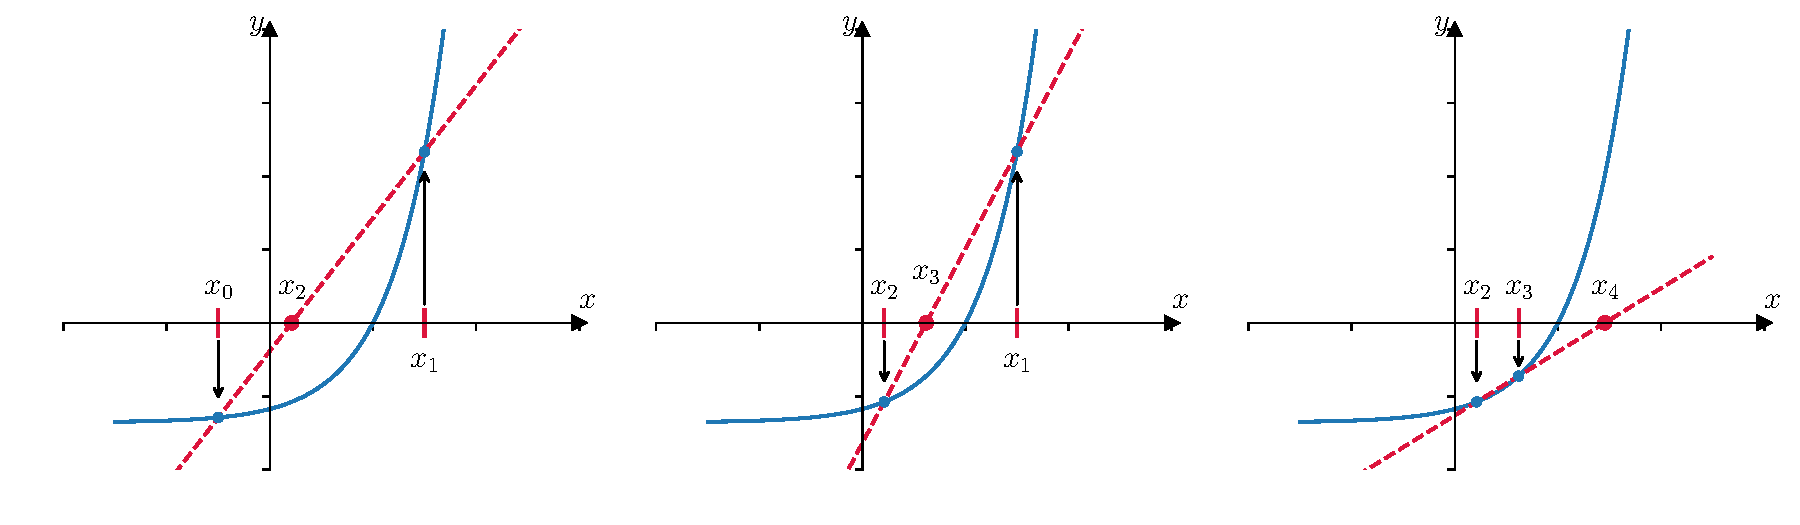
\includegraphics[width=\linewidth]{figures/ch2_secant1.pdf}  \label{fig:ch2_secant1}
\end{center}
\end{figure}

\noindent Notice that the approximation doesn't always stay on the same side of the function (blue curve), and in fact $x_4$ is even further away from the root than $x_3$. Sometimes it may take several iterations to settle down.


%%%%%%%%%%%%%%%%%%%%%%%%%%%%
%%%%%%%%%%%%%%%%%%%%%%%%%%%%
%%%%%%%%%%%%%%%%%%%%%%%%%%%%
%%%% Comparison %%%%
%%%%%%%%%%%%%%%%%%%%%%%%%%%%
%%%%%%%%%%%%%%%%%%%%%%%%%%%%
%%%%%%%%%%%%%%%%%%%%%%%%%%%%
\section{Comparison of methods}

For any of the methods we have studied, consider the error at each iteration $\epsilon_k = |x_k - \xi|$ where $\xi$ is a root. If we find that the following limit gives a constant 
\begin{align*}
\lim_{k\to\infty} \frac{\epsilon_{k+1}}{\epsilon_k^p} = C
\end{align*}
for some constant $C>0$, then we say the method has \textit{order of convergence} $p$. Note that $p$ is not forced to be an integer. This characterizes a rate of convergence and therefore lets us compare which method will reach a certain precision faster than another.

\subsection*{Bisection method}
We showed that the error in the bisection method is bounded
\begin{align*}
\epsilon_k \leq \frac{|b_0 - a_0|}{2^k}.
\end{align*}

\begin{align*}
\lim_{k\to\infty}\left( \dfrac{\frac{|b_0 - a_0|}{2^{k+1}}}{\frac{|b_0 - a_0|}{2^k}} \right)
=
\lim_{k\to\infty} \frac{1}{2}
=
\frac{1}{2}
\end{align*}


\subsection*{Newton method}
\subsection*{Secant method}


%%%%%%%%%%%%%%%%%%%%%%%%%%%%
%%%%%%%%%%%%%%%%%%%%%%%%%%%%
%%%%%%%%%%%%%%%%%%%%%%%%%%%%
%%%% Exercises %%%%
%%%%%%%%%%%%%%%%%%%%%%%%%%%%
%%%%%%%%%%%%%%%%%%%%%%%%%%%%
%%%%%%%%%%%%%%%%%%%%%%%%%%%%
\exercises{
\section{Exercises}

\exercice{Finding the intersection of $2\sin x=x$}
\begin{enumerate}[label=\alph*)]
	\item Sketch a graph of $y=2\sin x$ and $y=x$ in the domain $[-2\pi,2\pi]$. 
	
	\item Write a function $f(x)$ that has roots corresponding to the solutions of $2\sin x=x$.
	
	\item Use the Intermediate Value Theorem and the graph to find \textit{the number} of roots of $f(x)$, and give intervals surrounding them.
	
	\item Use the bisection algorithm to solve $2\sin x=x$ for as many iterations as needed       until the solution stops changing its first 4 decimal places. Do this for each       solution of $2\sin x=x$ that you found in part c.
	
	\item Define a function $g(x)$ so that we have an iterative scheme: $x_{k+1} = g(x_k)$ with fixed points at the roots of $f(x)$.
	
	\item Make a rough iteration figure exploring initial guesses $x_0$ and their subsequent      iterates using the iteration scheme of part e. Are there any unstable fixed-points? What value does $x_k$ converge to for initial $x_0$ where $\sin(x_0)>0$? What about initial $x_0$ where $\sin(x_0)<0$?
\end{enumerate}



\exercice{Finding the intersection of $\sin x=\cos x$}
\begin{enumerate}[label=\alph*)]
	\item Sketch a graph of $y=\sin x$ and $y=\cos x$ in the domain $[0,2\pi]$. 
	
	\item Write a function $f(x)$ that has roots corresponding to the solutions of $\sin x=\cos x$.
	
	\item Use the Intermediate Value Theorem and the graph to find \textit{the number} of roots of $f(x)$, and give intervals surrounding them.
	
	\item Use the bisection algorithm to solve $\sin x=x$ for as many iterations as needed       until the solution stops changing its first 4 decimal places. Do this for each       solution of $\sin x=\cos x$ that you found in part c.
\end{enumerate}



\exercice{Fixed-point analysis $g(x)=x(x^2-1)$}
\begin{enumerate}[label=\alph*)]
	\item How many fixed points, $\xi_k$, of $g(x)$ are there?
	
	\item Sketch a graph of $y=g(x)$ and $y=x$. Make rough iteration figures at different initial guesses $x_0$ on each side of the fixed points. Which fixed point(s) do you expect to be stable?
	
	\item Use the stability criterion on $|g(\xi_k)|$ to make a stability analysis of the fixed points.
\end{enumerate}



\exercice{Fixed-point analysis $f(x)=2e^{-x} + x - 2$}
\begin{enumerate}[label=\alph*)]
	\item Find 2 functions $g(x)$ for which the $x=g(x)$ has the same solutions as zeros of $f(x)$.
	
	\item Sketch separate graphs of the previous functions, as well as $y=2e^x$ and $y=2-x$ to get an intuition on the location of the roots or fixed points.
	
	\item Can you use Brouwer's theorem to guarantee the existence of any fixed points for either of the functions defined in part a?
	
	\item Make a stability analysis of the fixed points for both functions.
	
	\item For any stable fixed points, use the iterative scheme $x_{k+1}=g(x_k)$ for 5 iterations.
\end{enumerate}



\exercice{The intersection of $e^x=\cos x + 1$}
\begin{enumerate}[label=\alph*)]
	\item Sketch a graph of $y=e^x$ and $y=\cos x + 1$ in the domain $[-4\pi,4\pi]$. 
	
	\item Write a function $f(x)$ that has roots corresponding to the solutions of $e^x=\cos x + 1$.
	
	\item From the graph, how many positive roots and how many negative roots of $f(x)$ will there be?
	
	\item Use the Intermediate Value Theorem and the graph to prove there is a root of $f(x)$, for $x>0$.
	
	\item Use Netwon's method to propose an iterative scheme to find the roots of $f(x)$. Use this iterative scheme starting with $x_0=0$ to make a table of estimates $x_k$ for $k=0,1,\dots ,4$.
	
	\item Show that the function $g(x)=\log(\cos x + 1)$ gives an iterative scheme $x_{k+1} = g(x_k)$ with fixed points equal to the roots of $f(x)$. Determine a second function $h(x)$ which also satisfies these properties.
	
	\item Sketch a graph of $y=g(x)$ and $y=x$ in the domain $[-\pi,\pi]$. 
	
	\item Make a rough iteration figure exploring initial guesses x0 and their subsequent iterates using the iteration scheme with $g(x)$ of part f. Which fixed point(s) do you expect to be stable?
	
	\item Use the stability criterion on $|g(\xi_k)|$ to make a stability analysis of the fixed points $\xi_k \in [-\pi,\pi]$.
\end{enumerate}



\exercice{Fixed-point analysis $\log(x+2)=x^2$}
\begin{enumerate}[label=\alph*)]
	\item Sketch a graph of $y=\log(x+2)$ and $y=x^2$. 
	
	\item Write a function $f(x)$ that has roots corresponding to the solutions of $\log(x+2)=x^2$.
	
	\item From the graph, how many roots of $f(x)$ will there be?
	
	\item Use the Intermediate Value Theorem and the graph to locate the roots of $f(x)$.
	
	\item Use the Secant method to propose an iterative scheme to find the roots of $f(x)$. Use this iterative scheme twice, starting with $x_0=1$ and $x_1=2$ and then again with $x'_0=-1$ and $x_1=-1.5$ to make a table of estimates of $x_k$ and $x'_k$ until $k=4$.
	
	\item Show that the functions $g_1(x)=\exp(x^2)-2$ and $g_2(x)=( \log(x+2) )1/2$ give iterative schemes $x_{k+1} = g_i(x_k)$ with fixed points equal to the roots of $f(x)$.
	
	\item Sketch a graph of $y=g_1(x)$ and $y=x$. Sketch another graph of $y=g_2(x)$ and $y=x$. Can you use Brouwer's theorem to guarantee the existance of any fixed points for either $g_1(x)$ or $g_2(x)$?
	
	\item Make a rough iteration figure exploring initial guesses $x_0$ and their subsequent iterates using the iteration scheme with $g(x)$ of part f. Which fixed point(s) do you expect to be stable?
	
	\item Use the stability criterion on $|g_1(\xi_k)|$ and $|g_2(\xi_k)|$ to make a stability analysis of the fixed points $\xi_k$. For a stable fixed point of your choice, use the iterative scheme $x_{k+1}=g_i(x_k)$ to estimate the location of an intersection of $y=\log(x+2) $and $y=x_2$.
\end{enumerate}
}